\documentclass[twoside]{book}

% Packages required by doxygen
\usepackage{fixltx2e}
\usepackage{calc}
\usepackage{doxygen}
\usepackage[export]{adjustbox} % also loads graphicx
\usepackage{graphicx}
\usepackage[utf8]{inputenc}
\usepackage{makeidx}
\usepackage{multicol}
\usepackage{multirow}
\PassOptionsToPackage{warn}{textcomp}
\usepackage{textcomp}
\usepackage[nointegrals]{wasysym}
\usepackage[table]{xcolor}

% Font selection
\usepackage[T1]{fontenc}
\usepackage[scaled=.90]{helvet}
\usepackage{courier}
\usepackage{amssymb}
\usepackage{sectsty}
\renewcommand{\familydefault}{\sfdefault}
\allsectionsfont{%
  \fontseries{bc}\selectfont%
  \color{darkgray}%
}
\renewcommand{\DoxyLabelFont}{%
  \fontseries{bc}\selectfont%
  \color{darkgray}%
}
\newcommand{\+}{\discretionary{\mbox{\scriptsize$\hookleftarrow$}}{}{}}

% Page & text layout
\usepackage{geometry}
\geometry{%
  a4paper,%
  top=2.5cm,%
  bottom=2.5cm,%
  left=2.5cm,%
  right=2.5cm%
}
\tolerance=750
\hfuzz=15pt
\hbadness=750
\setlength{\emergencystretch}{15pt}
\setlength{\parindent}{0cm}
\setlength{\parskip}{3ex plus 2ex minus 2ex}
\makeatletter
\renewcommand{\paragraph}{%
  \@startsection{paragraph}{4}{0ex}{-1.0ex}{1.0ex}{%
    \normalfont\normalsize\bfseries\SS@parafont%
  }%
}
\renewcommand{\subparagraph}{%
  \@startsection{subparagraph}{5}{0ex}{-1.0ex}{1.0ex}{%
    \normalfont\normalsize\bfseries\SS@subparafont%
  }%
}
\makeatother

% Headers & footers
\usepackage{fancyhdr}
\pagestyle{fancyplain}
\fancyhead[LE]{\fancyplain{}{\bfseries\thepage}}
\fancyhead[CE]{\fancyplain{}{}}
\fancyhead[RE]{\fancyplain{}{\bfseries\leftmark}}
\fancyhead[LO]{\fancyplain{}{\bfseries\rightmark}}
\fancyhead[CO]{\fancyplain{}{}}
\fancyhead[RO]{\fancyplain{}{\bfseries\thepage}}
\fancyfoot[LE]{\fancyplain{}{}}
\fancyfoot[CE]{\fancyplain{}{}}
\fancyfoot[RE]{\fancyplain{}{\bfseries\scriptsize Generated by Doxygen }}
\fancyfoot[LO]{\fancyplain{}{\bfseries\scriptsize Generated by Doxygen }}
\fancyfoot[CO]{\fancyplain{}{}}
\fancyfoot[RO]{\fancyplain{}{}}
\renewcommand{\footrulewidth}{0.4pt}
\renewcommand{\chaptermark}[1]{%
  \markboth{#1}{}%
}
\renewcommand{\sectionmark}[1]{%
  \markright{\thesection\ #1}%
}

% Indices & bibliography
\usepackage{natbib}
\usepackage[titles]{tocloft}
\setcounter{tocdepth}{3}
\setcounter{secnumdepth}{5}
\makeindex

% Hyperlinks (required, but should be loaded last)
\usepackage{ifpdf}
\ifpdf
  \usepackage[pdftex,pagebackref=true]{hyperref}
\else
  \usepackage[ps2pdf,pagebackref=true]{hyperref}
\fi
\hypersetup{%
  colorlinks=true,%
  linkcolor=blue,%
  citecolor=blue,%
  unicode%
}

% Custom commands
\newcommand{\clearemptydoublepage}{%
  \newpage{\pagestyle{empty}\cleardoublepage}%
}

\usepackage{caption}
\captionsetup{labelsep=space,justification=centering,font={bf},singlelinecheck=off,skip=4pt,position=top}

%===== C O N T E N T S =====

\begin{document}

% Titlepage & ToC
\hypersetup{pageanchor=false,
             bookmarksnumbered=true,
             pdfencoding=unicode
            }
\pagenumbering{roman}
\begin{titlepage}
\vspace*{7cm}
\begin{center}%
{\Large My Project }\\
\vspace*{1cm}
{\large Generated by Doxygen 1.8.11}\\
\end{center}
\end{titlepage}
\clearemptydoublepage
\tableofcontents
\clearemptydoublepage
\pagenumbering{arabic}
\hypersetup{pageanchor=true}

%--- Begin generated contents ---
\chapter{File Index}
\section{File List}
Here is a list of all files with brief descriptions\+:\begin{DoxyCompactList}
\item\contentsline{section}{\hyperlink{Lab1_8c}{Lab1.\+c} }{\pageref{Lab1_8c}}{}
\end{DoxyCompactList}

\chapter{File Documentation}
\hypertarget{HW9_8cpp}{}\section{H\+W9.\+cpp File Reference}
\label{HW9_8cpp}\index{H\+W9.\+cpp@{H\+W9.\+cpp}}
{\ttfamily \#include $<$iostream$>$}\\*
{\ttfamily \#include $<$vector$>$}\\*
Include dependency graph for H\+W9.\+cpp\+:
\nopagebreak
\begin{figure}[H]
\begin{center}
\leavevmode
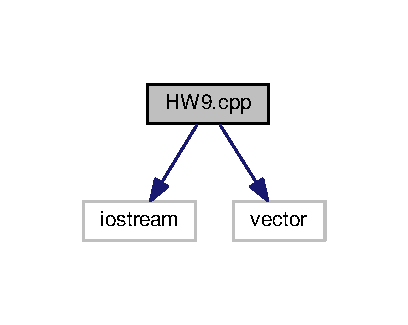
\includegraphics[width=196pt]{HW9_8cpp__incl}
\end{center}
\end{figure}
\subsection*{Functions}
\begin{DoxyCompactItemize}
\item 
void \hyperlink{HW9_8cpp_ae44c5d3a586f372d9c366ad9bec64e0c}{permutation} (vector$<$ int $>$ v, vector$<$ int $>$ $\ast$pv, int n)
\item 
void \hyperlink{HW9_8cpp_afcd58f6b3dcd6630a12fa667239b638b}{fill} (vector$<$ int $>$ $\ast$pv, int start, int end, vector$<$ int $>$ v, int num)
\item 
vector$<$ int $>$ \hyperlink{HW9_8cpp_acca24749d888f73c0a7fe113d849dfae}{perm} (vector$<$ int $>$ v, int n)
\item 
void \hyperlink{HW9_8cpp_a9f8419e439090ecd27f2c5d086efb2ad}{swap} (vector$<$ int $>$ \&v, int current, int other)
\item 
void \hyperlink{HW9_8cpp_a6562deebd6a84f141eabc853a955f835}{display} (vector$<$ int $>$ $\ast$pv)
\item 
int \hyperlink{HW9_8cpp_ae66f6b31b5ad750f1fe042a706a4e3d4}{main} ()
\end{DoxyCompactItemize}


\subsection{Function Documentation}
\index{H\+W9.\+cpp@{H\+W9.\+cpp}!display@{display}}
\index{display@{display}!H\+W9.\+cpp@{H\+W9.\+cpp}}
\subsubsection[{\texorpdfstring{display(vector$<$ int $>$ $\ast$pv)}{display(vector< int > *pv)}}]{\setlength{\rightskip}{0pt plus 5cm}void display (
\begin{DoxyParamCaption}
\item[{vector$<$ int $>$ $\ast$}]{pv}
\end{DoxyParamCaption}
)}\hypertarget{HW9_8cpp_a6562deebd6a84f141eabc853a955f835}{}\label{HW9_8cpp_a6562deebd6a84f141eabc853a955f835}

\begin{DoxyCode}
99 \{
100    vector<int> temp;
101    \textcolor{keywordflow}{for}(\textcolor{keywordtype}{int} k = 0; k < pv->size(); k++)
102    \{
103       temp = pv[k];
104       cout << \textcolor{stringliteral}{"\{ "};
105       \textcolor{keywordflow}{for}(\textcolor{keywordtype}{int} j = 0; j < pv[k].size(); j++)
106          cout << temp[j] << \textcolor{stringliteral}{" "};
107       cout << \textcolor{stringliteral}{"\}"} << endl;
108    \}
109 \}
\end{DoxyCode}
\index{H\+W9.\+cpp@{H\+W9.\+cpp}!fill@{fill}}
\index{fill@{fill}!H\+W9.\+cpp@{H\+W9.\+cpp}}
\subsubsection[{\texorpdfstring{fill(vector$<$ int $>$ $\ast$pv, int start, int end, vector$<$ int $>$ v, int num)}{fill(vector< int > *pv, int start, int end, vector< int > v, int num)}}]{\setlength{\rightskip}{0pt plus 5cm}void fill (
\begin{DoxyParamCaption}
\item[{vector$<$ int $>$ $\ast$}]{pv, }
\item[{int}]{start, }
\item[{int}]{end, }
\item[{vector$<$ int $>$}]{v, }
\item[{int}]{num}
\end{DoxyParamCaption}
)}\hypertarget{HW9_8cpp_afcd58f6b3dcd6630a12fa667239b638b}{}\label{HW9_8cpp_afcd58f6b3dcd6630a12fa667239b638b}

\begin{DoxyCode}
64 \{
65    \textcolor{keywordtype}{int} p = 1;
66    \textcolor{keywordflow}{for}(\textcolor{keywordtype}{int} k = start; k <= end; k++)
67    \{
68       \textcolor{keywordflow}{for}(\textcolor{keywordtype}{int} j = 0; j < v.size(); j++)
69          pv[k].push\_back(v[j]);
70    \}
71 
72    \textcolor{keywordflow}{for}(\textcolor{keywordtype}{int} m = start+1; m <= end; m++)
73    \{
74       pv[m] = \hyperlink{HW9_8cpp_acca24749d888f73c0a7fe113d849dfae}{perm}(pv[m], p);
75       p++;
76    \}
77 \}
\end{DoxyCode}


Here is the call graph for this function\+:
\nopagebreak
\begin{figure}[H]
\begin{center}
\leavevmode
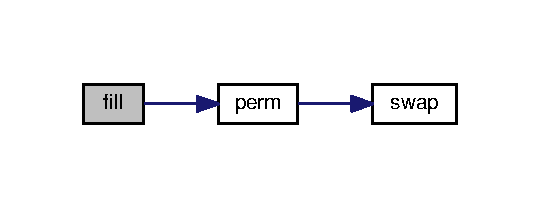
\includegraphics[width=259pt]{HW9_8cpp_afcd58f6b3dcd6630a12fa667239b638b_cgraph}
\end{center}
\end{figure}


\index{H\+W9.\+cpp@{H\+W9.\+cpp}!main@{main}}
\index{main@{main}!H\+W9.\+cpp@{H\+W9.\+cpp}}
\subsubsection[{\texorpdfstring{main()}{main()}}]{\setlength{\rightskip}{0pt plus 5cm}int main (
\begin{DoxyParamCaption}
{}
\end{DoxyParamCaption}
)}\hypertarget{HW9_8cpp_ae66f6b31b5ad750f1fe042a706a4e3d4}{}\label{HW9_8cpp_ae66f6b31b5ad750f1fe042a706a4e3d4}

\begin{DoxyCode}
15 \{
16    vector<int> list;
17    \textcolor{comment}{//vector<vector<int> > perm\_list;                                                                       
                                                                                                       }
18    \textcolor{keywordtype}{int} num;
19    \textcolor{keywordtype}{char} choice = \textcolor{charliteral}{'y'};
20    \textcolor{keywordflow}{while}(choice == \textcolor{charliteral}{'y'} || choice == \textcolor{charliteral}{'Y'})
21    \{
22       cout << \textcolor{stringliteral}{"Please enter an integer: "};
23       cin >> num;
24       list.push\_back(num);
25       cout << \textcolor{stringliteral}{"Would you like to add another number? Enter Y or y to do so, and any other character to
       quit: "};
26       cin >> choice;
27    \}
28    \textcolor{keywordtype}{int} perm\_num = 0;
29    \textcolor{keywordflow}{for}(\textcolor{keywordtype}{int} k = 1; k < list.size(); k++)
30       perm\_num = perm\_num*k;
31    vector<int>* p = \textcolor{keyword}{new} vector<int>[perm\_num];
32    \hyperlink{HW9_8cpp_ae44c5d3a586f372d9c366ad9bec64e0c}{permutation}(list, p, 0);
33    \hyperlink{HW9_8cpp_a6562deebd6a84f141eabc853a955f835}{display}(p);
34    \textcolor{keyword}{delete} [] p;
35    \textcolor{keywordflow}{return} 0;
36 \}
\end{DoxyCode}


Here is the call graph for this function\+:
\nopagebreak
\begin{figure}[H]
\begin{center}
\leavevmode
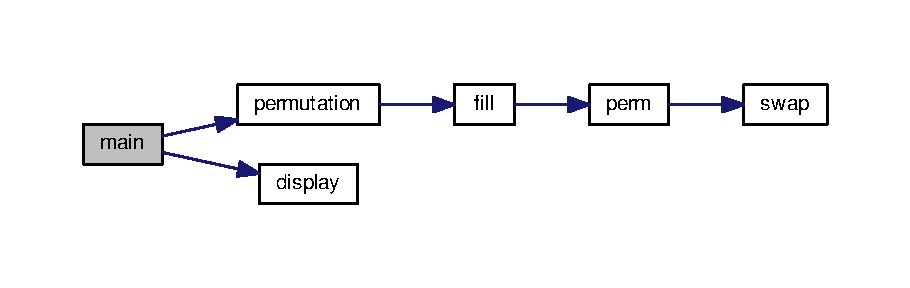
\includegraphics[width=350pt]{HW9_8cpp_ae66f6b31b5ad750f1fe042a706a4e3d4_cgraph}
\end{center}
\end{figure}


\index{H\+W9.\+cpp@{H\+W9.\+cpp}!perm@{perm}}
\index{perm@{perm}!H\+W9.\+cpp@{H\+W9.\+cpp}}
\subsubsection[{\texorpdfstring{perm(vector$<$ int $>$ v, int n)}{perm(vector< int > v, int n)}}]{\setlength{\rightskip}{0pt plus 5cm}vector$<$ int $>$ perm (
\begin{DoxyParamCaption}
\item[{vector$<$ int $>$}]{v, }
\item[{int}]{n}
\end{DoxyParamCaption}
)}\hypertarget{HW9_8cpp_acca24749d888f73c0a7fe113d849dfae}{}\label{HW9_8cpp_acca24749d888f73c0a7fe113d849dfae}

\begin{DoxyCode}
80 \{
81    \textcolor{keywordtype}{int} q = 1;
82    \textcolor{keywordflow}{for}(\textcolor{keywordtype}{int} k = 0; k < n; k++)
83    \{
84       \hyperlink{HW9_8cpp_a9f8419e439090ecd27f2c5d086efb2ad}{swap}(v, 0, q);
85       q++;
86       \textcolor{keywordflow}{if}(q > v.size())
87          q = 1;
88    \}
89 \}
\end{DoxyCode}


Here is the call graph for this function\+:
\nopagebreak
\begin{figure}[H]
\begin{center}
\leavevmode
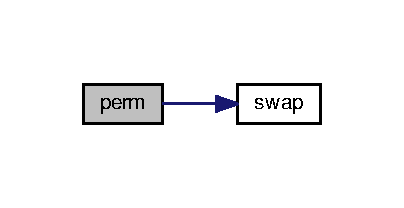
\includegraphics[width=194pt]{HW9_8cpp_acca24749d888f73c0a7fe113d849dfae_cgraph}
\end{center}
\end{figure}


\index{H\+W9.\+cpp@{H\+W9.\+cpp}!permutation@{permutation}}
\index{permutation@{permutation}!H\+W9.\+cpp@{H\+W9.\+cpp}}
\subsubsection[{\texorpdfstring{permutation(vector$<$ int $>$ v, vector$<$ int $>$ $\ast$pv, int n)}{permutation(vector< int > v, vector< int > *pv, int n)}}]{\setlength{\rightskip}{0pt plus 5cm}void permutation (
\begin{DoxyParamCaption}
\item[{vector$<$ int $>$}]{v, }
\item[{vector$<$ int $>$ $\ast$}]{pv, }
\item[{int}]{n}
\end{DoxyParamCaption}
)}\hypertarget{HW9_8cpp_ae44c5d3a586f372d9c366ad9bec64e0c}{}\label{HW9_8cpp_ae44c5d3a586f372d9c366ad9bec64e0c}

\begin{DoxyCode}
39 \{
40    \textcolor{keywordtype}{int} perm\_num = 1, p = 0;
41    std::vector<int>::iterator it;
42    \textcolor{keywordflow}{for}(\textcolor{keywordtype}{int} k = 1; k < v.size(); k++)
43       perm\_num = perm\_num*k;
44    \textcolor{keywordtype}{int} num = perm\_num/v.size();
45 
46    \textcolor{keywordflow}{if}(n < num)
47       \hyperlink{HW9_8cpp_ae44c5d3a586f372d9c366ad9bec64e0c}{permutation}(v, pv, ++n);
48    n--;
49 
50    vector<int> temp = v;
51    temp.erase(temp.begin() + n);
52    \textcolor{keywordtype}{int} m = n*num;
53    \textcolor{keywordtype}{int} start = m-1, end = m+num-1;
54    \hyperlink{HW9_8cpp_afcd58f6b3dcd6630a12fa667239b638b}{fill}(pv, start, end, temp, num);
55 
56    \textcolor{keywordflow}{for}(\textcolor{keywordtype}{int} q = start; q <= end; q++)
57    \{
58       it = pv[q].begin();
59       pv[q].insert(it, 1, v[n]);
60    \}
61 \}
\end{DoxyCode}


Here is the call graph for this function\+:
\nopagebreak
\begin{figure}[H]
\begin{center}
\leavevmode
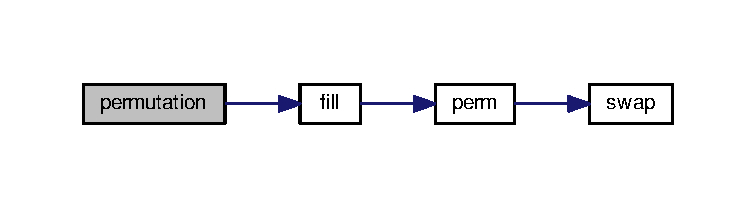
\includegraphics[width=350pt]{HW9_8cpp_ae44c5d3a586f372d9c366ad9bec64e0c_cgraph}
\end{center}
\end{figure}


\index{H\+W9.\+cpp@{H\+W9.\+cpp}!swap@{swap}}
\index{swap@{swap}!H\+W9.\+cpp@{H\+W9.\+cpp}}
\subsubsection[{\texorpdfstring{swap(vector$<$ int $>$ \&v, int current, int other)}{swap(vector< int > &v, int current, int other)}}]{\setlength{\rightskip}{0pt plus 5cm}void swap (
\begin{DoxyParamCaption}
\item[{vector$<$ int $>$ \&}]{v, }
\item[{int}]{current, }
\item[{int}]{other}
\end{DoxyParamCaption}
)}\hypertarget{HW9_8cpp_a9f8419e439090ecd27f2c5d086efb2ad}{}\label{HW9_8cpp_a9f8419e439090ecd27f2c5d086efb2ad}

\begin{DoxyCode}
92 \{
93    \textcolor{keywordtype}{int} temp = v[current];
94    v[current] = v[other];
95    v[other] = temp;
96 \}
\end{DoxyCode}

%--- End generated contents ---

% Index
\backmatter
\newpage
\phantomsection
\clearemptydoublepage
\addcontentsline{toc}{chapter}{Index}
\printindex

\end{document}
